% Preamble
% ---
\documentclass{article}

% Packages
% ---
\usepackage{amsmath} % Advanced math typesetting
\usepackage[utf8]{inputenc} % Unicode support (Umlauts etc.)
\usepackage{hyperref} % Add a link to your document
\hypersetup{
    colorlinks=true,
    linkcolor=black,
    filecolor=black,
    citecolor=blue,
    urlcolor=blue,
}
\usepackage{graphicx} % Add pictures to your document
\usepackage{listings} % Source code formatting and highlighting
\usepackage{framed} % Source code formatting and highlighting
\usepackage{appendix} % Source code formatting and highlighting
\usepackage{csquotes} % Pretty quotes
\usepackage[automake]{glossaries}
\usepackage[letterpaper, portrait, margin=1.5in]{geometry}
\usepackage{multicol}

\graphicspath{ {images/} }

\makeglossary

%*******************************
%**** Begin Glossary Section *****
%*******************************

\newglossaryentry{sentinel}
{
    name={Sentinel},
    description={A Sentinel is a heuristic witness. It observes heuristics and vouches for the certainty and accuracy of them by producing temporal ledgers. The most important aspect of a Sentinel is that it produces ledgers that Diviners can be certain came from the same source by adding Proof of Origin to them}
}

\newglossaryentry{bridge}
{
    name={Bridge},
    description={A Bridge is a heuristic transcriber. It securely relays heuristic ledgers from Sentinels to Diviners. The most important aspect of a Bridge is that a Diviner can be sure that the heuristic ledgers that are received from a Bridge have not been altered in any way. The second most important aspect of a Bridge is that they add an additional Proof of Origin metadata}
}

\newglossaryentry{archivist}
{
    name={Archivist},
    description={An Archivist stores heuristics as a part of the decentralized data set with the goal of having all historical ledgers stored, but without that requirement. Even if some data is lost or becomes temporarily unavailable, the system continues to function, just with reduced accuracy. Archivists also index ledgers so that they can return a string of ledger data if needed. Archivists store raw data only and get paid solely for retrieval of the data. Storage is always free}
}

\newglossaryentry{diviner}
{
    name={Diviner},
    description={A Diviner answers a given query by analyzing historical data that has been stored by the XYO Network. Heuristics stored in the XYO Network must have a high level of Proof of Origin to determine the validity and accuracy of the heuristic. A Diviner obtains and delivers an answer by judging the witness based on its Proof of Origin. Given that the XYO Network is a trustless system, Diviners must be incentivized to provide honest analyses of heuristics. Unlike Sentinels and Bridges, Diviners use Proof of Work to add answers to the blockchain}
}

\newglossaryentry{webble}
{
    name={webble},
    description={Everything in the world is defined spatially by its \textit{X,Y,Z,T} coordinate and nothing can leave that space. Objects are thus confined to ``webbubbles'', or what are referred to as \textit{webbles}.}
}

\newglossaryentry{gas}
{
    name={gas},
    description={The cost of a transaction (i.e. query) in the form of XYO Tokens}
}

\newglossaryentry{proof-of-origin}
{
    name={Proof of Origin},
    description={Proof of Origin is the key to verifying that ledgers flowing into the XYO Network are valid. A unique ID for source of data is not practical since it can be forged. Private key signing is not practical since most parts of the XYO Network are difficult or impossible to physically secure, thus the potential for a bad actor to steal a private key is too feasible. To solve this, XYO Network uses Transient Key Chaining. The benefit of this is that it is impossible to falsify the chain of origin for data. However, once the chain is broken, it is broken forever and cannot be continued, rendering it an island}
}

\newglossaryentry{proof-of-work}
{
    name={Proof of Work},
    description={Proof of Work is a piece of data that satisfies certain requirements, is difficult to produce (i.e. costly, time-consuming), but easy for others to verify. Producing a Proof of Work can be a random process with a low probability of generation so that rigorous trial and error is required on average before a valid Proof of Work is created}
}

\newglossaryentry{bound-witness}
{
    name={Bound Witness},
    description={Bound Witness is a concept achieved by the existence of a bidirectional heuristic. Given that an untrusted source of data for the use of digital contract resolution (an oracle) is not useful, there is a substantial increase in certainty of the data provided by the establishment of such a heuristic. The primary bidirectional heuristic is proximity since both parties can validate the occurrence and range of an interaction by cosigning the interaction. This allows for a zero-knowledge proof that the two nodes were in proximity of each other.}
}

\newglossaryentry{smart-contract}
{
    name={smart contract},
    description={A protocol coined by Nick Szabo before Bitcoin, purportedly in 1994 (which is why some believe him to be Satoshi Nakamoto, the mystical and unknown inventor of Bitcoin). The idea behind smart contracts is to codify a legal agreement in a program and to have decentralized computers execute its terms, instead of humans having to interpret and act on contracts. Smart contracts collapse money (e.g. Ether) and contracts into the same concept. Being that smart contracts are deterministic (like computer programs) and fully transparent and readable, they serve as a powerful way to replace middle-men and brokers}
}

\newglossaryentry{cryptoeconomics}
{
    name={cryptoeconomics},
    plural={cryptoeconomic},
    description={A formal discipline that studies protocols that govern the production, distribution, and consumption of goods and services in a decentralized digital economy. Cryptoeconomics is a practical science that focuses on the design and characterization of these protocols}
}

\newglossaryentry{xyo-network}
{
    name={XYO Network},
    description={XYO Network stands for ``XY Oracle Network.'' It is comprised of the entire system of XYO enabled components/nodes that include Sentinels, Bridges, Archivists, and Diviners. The primary function of the XYO Network is to act as a portal by which digital smart contracts can be executed through real world geo-location confirmations}
}

\newglossaryentry{certainty}
{
    name={certainty},
    description={A measure of the likelihood that a data point or heuristic is free from corruption or tampering}
}

\newglossaryentry{accuracy}
{
    name={accuracy},
    description={A measure of confidence that a data point or heuristic is within a specific margin of error}
}

\newglossaryentry{oracle}
{
    name={oracle},
    description={A part of a DApp (decentralized application) system that is responsible for resolving a digital contract by providing an answer with accuracy and certainty. The term ``oracle'' originates from cryptography where it signifies a truly random source (e.g. of a random number). This provides the necessary gate from a crypto equation to the world beyond. Oracles feed smart contracts information from beyond the chain (the real world, or off-chain). Oracles are interfaces from the digital world to the real world. As a morbid example, consider a contract for a Last Will \& Testament. A Will's terms are executed upon confirmation that the testator is deceased. An oracle service could be built to trigger a Will by compiling and aggregating relevant data from official sources. The oracle could then be used as a feed or end-point for a smart contract to call out to in order to check whether or not the person is deceased}
}

\newglossaryentry{heuristic}
{
    name={heuristic},
    description={A data point about the real world relative to the position of a Sentinel (proximity, temperature, light, motion, etc...)}
}

\newglossaryentry{transient-key-chain}
{
    name={Transient Key Chain},
    description={A Transient Key Chain links a series of data packets using Transient Key Cryptography}
}

\newglossaryentry{best-answer}
{
    name={Best Answer},
    description={We define the Best Answer as the single answer, amongst a list of Answer Candidates, that returns the highest validity score and has a higher accuracy score than the minimum required accuracy.}
}

\newglossaryentry{best-answer-score}
{
    name={Best Answer Score},
    description={A score generated by a Best Answer Algorithm that ranks the quality of the score.  The higher the score, the better it is, per the algorithm.  This score is used to determine which answer is better given two analyzed answers}
}

\newglossaryentry{best-answer-algorithm}
{
    name={Best Answer Algorithm},
    description={An algorithm used to generate Best Answer Scores when a Diviner chooses an answer.  The XYO Network permits the addition of specialized algorithms and allows the customer to specify which algorithm to use.  It is required that this algorithm will result in the same score when run on any Diviner given the same data set}
}

\newglossaryentry{origin-chain-score}
{
    name={Origin Chain Score},
    description={The score assigned to an Origin Chain to determine its credibility. This assessment takes length, tangle, overlap, and redundancy into consideration}
}

\newglossaryentry{proof-of-origin-chain}
{
    name={Proof of Origin Chain},
    description={A Transient Key Chain that links together a series of Bound Witness heuristic ledger entries}
}

\newglossaryentry{origin-tree}
{
    name={Origin Tree},
    description={A data set of ledger entries taken from various Origin Chains to establish the origin of a heuristic ledger entry with a specified level of certainty}
}

\newglossaryentry{crypto-location}
{
    name={crypto-location},
    description={The realm of cryptographic location technology}
}

\newglossaryentry{trustless}
{
    name={trustless},
    description={A characteristic where all parties in a system can reach a consensus on what the canonical truth is. Power and trust is distributed (or shared) among the network’s stakeholders (e.g. developers, miners, and consumers), rather than concentrated in a single individual or entity (e.g. banks, governments, and financial institutions). This is a common term that can be easily misunderstood. Blockchains don’t actually eliminate trust. What they do is minimize the amount of trust required from any single actor in the system. They do this by distributing trust among different actors in the system via an economic game that incentivizes actors to cooperate with the rules defined by the protocol}
}

\newglossaryentry{xyomainchain}
{
    name={XYOMainChain},
    description={An immutable blockchain in the XYO Network that stores query transactions along with data gathered from Diviners and their associated origin score}
}

\newglossaryentry{xyo-miner}
{
    name={XYO Miner},
    description={Sentinels, Bridges, Archivists, and Deviners who take part in answering queries to the XYO Network in an XYO crypto-location mining pool}
}

\newglossaryentry{ideal-state}   
{
    name={ideal-state},
    description={The location-verification standard in an XYO crypto-location mining pool. It can be voted on amongst other XYO miners in the XYO Network system votes to increase or decrease this standard}
}

\newglossaryentry{proof-of-eligibility}
{
	name={Proof of Eligibility},
    description={Addresses the dilemma of eligibility verification and potential cost-based attacks through a reorganization of the steps required to complete the transaction}
}

\newglossaryentry{candidate}
{
    name={Candidate},
    description={A wallet address under consideration for a transaction}
}

\newglossaryentry{contract-caller}
{
    name={contract caller},
    description={An entity that initiates a smart contract, on the receiving end of the contract holder's input}
}

\newglossaryentry{contract-holder}
{
	name={contract holder},
    description={An entity that controls a smart contract, on the receiving end of the contract caller's input}
}

\newglossaryentry{cost-based-attack}
{
    name={cost-based attack},
    description={A malicious attempt by one entity to increase incurred costs for another, often through high-volume data input for a costly process with little to no cost to the attacker}
}

\newglossaryentry{transaction}
{
	name={transaction},
    description={The necessary requirements and entire process involved in the execution of a smart contract}
}

\newglossaryentry{transaction-architecture}
{
	name={transaction architecture},
    description={The basic structure of a transaction, often a list of steps that result in an executed smart contract}
}

\newacronym{pow}{PoW}{Proof of Work}

\newacronym{poo}{PoO}{Proof of Origin}

\newacronym{xy-oracle-network}{XY Oracle Network}{XYO Network}

\newacronym{poe}{PoE}{Proof of Eligibility}

\newacronym{xyo}{XYO}{XY Oracle Network}

\title {The XY Oracle Network: Proof of Eligibility Transactions and XYO Token Sale Logistics}


\author{
    Arie Trouw
        \thanks{XYO Network, \texttt{arie.trouw@xyo.network}}
}

\date{March 2018}

\begin{document}
\maketitle

\begin{center}
\line(1,0){50}
\end{center}

%Abstract Section
\begin{abstract}
Most \glspl{smart-contract} only allow certain entities to be eligible to engage in \glspl{transaction}. There is an incurred burden and expense with the eligibility validation process of the \gls{contract-caller} that can expose \glspl{contract-holder} to high drop-off rates and \glspl{cost-based-attack}. Traditionally, confirmation of eligibility verification is often saved only to external servers, not to the smart contracts themselves, leaving the potential for contract holders to incur future risks. The \Gls{xy-oracle-network} provides a solution to the risk assumed by contract holders by establishing the architecture for \textbf{\Gls{poe}} transactions. The implementation of \acrshort{poe} allows the contract caller to validate their eligibility \textit{after} initiating a smart contract, which confirms their position in contracts that are temporally sensitive and/or have limited availability. Additionally, transactions with Proof of Eligibility save affirmation of eligibility verification directly to the smart contract in order to prevent any further liability to the contract holder. The XYO Network employs Proof of Eligibility transactions to minimize liability and risk to Token buyers in its limited volume and variably priced XYO Token Sale. The XYO Network also adopts the Proof of Eligibility structure for all XYO Token Sale transactions due to its requirement for Token buyers to have KYC ("Know Your Customer") eligibility verification.
%after initiating the contract, but prior to contract execution and receipt of the benefit of the transaction.

\begin{center}
\line(1,0){50}
\end{center}
\end{abstract}

%Introduction
\section{Introduction}
The verification for \Gls{smart-contract} eligibility is most frequently implemented to selectively permit transactions between \glspl{contract-holder} and eligible \glspl{contract-caller}. The requirement of contract caller eligibility verification ensures safety and control for contract holders, but results in higher costs for contract holders who must pay to invoke this process. Eligibility verification is burdensome and complex for contract callers, which can lead to their decreased commitment and higher drop-off rate. Finally, contract holders can also be hurt by \glspl{cost-based-attack}, where entities interested in increasing costs to contract holders continuously provide irrelevant or false data in order to initiate the process of eligibility verification, without the intent to complete a transaction. This type of attack incurs very little cost to the attacker, but high costs to the contract holder.

\Gls{proof-of-eligibility} mitigates the dilemma involved with historical implementations of eligibility verification and potential cost-based attacks through a reorganization of the steps required to complete a transaction. Traditional \gls{transaction-architecture} prioritizes the process of eligibility verification over the initiation of the transaction, which negatively impacts both the contract caller and the contract holder. Contract callers are deterred sooner in the transaction for two reasons: the eligibility verification process is complex and laborious, and the duration of the third-party eligibility verification procedure threatens their opportunity to execute the contract. Contract holders experience greater contract caller drop-off rates while exposing themselves to cost-based attacks due to the low cost for the contract caller to input data for verification. The \Gls{xyo-network}'s \acrshort{poe} model for transaction architecture prioritizes the \textit{initiation} of the smart contract over the overall \textit{process} of eligibility verification. Initiating a contract earlier in the overall transaction process both preserves the original transaction order in the blockchain and timestamps the initiation of the contract (which is particularly useful for contract callers in cases of smart contracts that are temporally sensitive and/or have limited availability). Additionally, initiation prior to verification increases the contract caller's commitment to the transaction earlier in the funnel, which decreases their drop-off rates and deters them from performing cost-based attacks.

The usage of \Gls{proof-of-eligibility} in smart contract transactions provides the benefits of preservation of transaction order, confirmation of contract initiation, and increased contract caller commitment.

\begin{center}
\line(1,0){50}
\end{center}

%Architecture
\section{Historical vs. XYO Network's Implementation of Transaction Architecture}
Historical implementations of \gls{smart-contract} \gls{transaction-architecture} prioritize eligibility verification prior to smart contract initiation and ultimately save the eligibility verification data to a server. This approach is susceptible to \glspl{cost-based-attack}, higher drop-off rates, and loss of data (should the server be compromised). The \Gls{xyo-network}'s implementation of \Gls{proof-of-eligibility} restructures transaction architecture and prioritizes transaction initiation over the eligibility verification process. The requirement of the \gls{contract-caller} to initiate the contract \textit{before} the verification process increases their commitment to the contract and disincentivizes them to abandon or attack the \gls{contract-holder}. Additionally, PoE transaction architecture saves verification data directly to the smart contract itself, which is far more secure than a private server.

\subsection{Diagram and Comparison}
The following diagram emphasizes the prioritization of eligibility verification vs. smart contract initiation between the historical and \Gls{xyo-network}'s transation architecture. The steps in each process are outlined in order and reveal that while a \Gls{proof-of-eligibility} transaction is more complex, it benefits from the separation of the smart contract execution into an initialization step and a completion step.  This separation solidifies contract caller commitment earlier in the structure. For added security, a \acrshort{poe} transaction saves verification data directly to the smart contract instead of to a server.

\begin{multicols}{2}

\begin{center}
\textbf{Historical Architecture Process}
\end{center}
\begin{enumerate}
\item Introduce \Gls{contract-caller}-facing platform
\item Begin eligibility verification
\item Send caller to third-party for eligibility verification
\item Store caller eligibility
\item Return to customer-facing platform with eligibility verification
\item \textbf{Execute contract}
\item \textbf{Save verification data to server}
\end{enumerate}

\columnbreak

\begin{center}
\textbf{PoE Architecture Process}
\end{center}
\begin{enumerate}
\item Introduce \Gls{contract-caller}-facing platform
\item \textbf{Initiate transaction}
\item Begin eligibility verification
\item Send caller to third-party for eligibility verification
\item Store caller eligibility
\item Return to customer-facing platform with eligibility verification
\item \textbf{Complete contract}
\item \textbf{Save verification data to smart contract}
\end{enumerate}

\end{multicols}

\vfill

\begin{multicols}{2}
\begin{center}
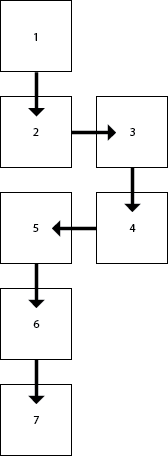
\includegraphics[width=100pt] {archHist.png}\\
\vspace{4mm}
\vfill
\textbf{Figure 1.}  Historical Architecture
\end{center}

\columnbreak

\begin{center}
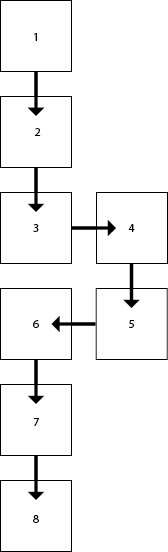
\includegraphics[width=90pt] {archPoE.png}\\
\vspace{4mm}
\vfill
\textbf{Figure 1.} PoE Architecture
\end{center}

\end{multicols}

\begin{center}
\line(1,0){50}
\end{center}

\section {Example: XYO Token Purchase with Ether}
A purchase of XYO Tokens with Ether exemplifies the benefits of a transaction utilizing \Gls{proof-of-eligibility} due to the complexity of the XYO Token Sale's pricing structure. The XYO Token Sale employs a pricing model that is calculated from a token availability-based equation designed by the \Gls{xyo-network}. This temporally sensitive and availability-based pricing makes a Proof of Eligibility-based \gls{transaction-architecture} particularly favorable to both the XYO Network and \glspl{contract-caller} who wish to contribute Ether to purchase XYO Tokens. The dependence of price on real-time token availability renders confirmation of contract initiation and maintenance of transaction order crucial.

During any Token Sale that employs price variability and/or volume-sensitivity, it is imperative for a contract caller's position in the order of transactions to be maintained. When a Token price is contingent on the number of Tokens sold to-date, the longer a \gls{contract-caller} waits to purchase Tokens with Ether, the higher the Token price (unless the Token price became fixed at an earlier point). If the Token price in Ether becomes fixed, maintenance of transaction order in relation to others will still be important to contract callers, since a contract initiation that occurs after the final token is sold will result in a a zero-Token return.

\vfill

\begin{multicols}{2}
\begin{center}
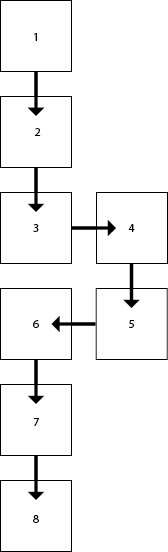
\includegraphics[width=100pt] {archXYOTokenSale.png}\\
\vspace{4mm}
\vfill
\textbf{Figure 1.}  Contract Caller purchases XYO Tokens with Ether
\end{center}

\columnbreak

\begin{center}
\textbf{Process}
\end{center}
\begin{enumerate}
\item Customer sends Ether payment for XYO Tokens to the \gls{smart-contract}.
\item The smart contract records the \gls{transaction} by adding the incoming address to a list and associates it with the number of XYO Tokens that are to be distributed to the customer.  The contributed Ether is added to the value of the contract.
\item The customer completes the verification process (KYC and/or AML).
\item An authorized wallet calls the contract to confirm that the customer has passed eligibility verification.
\item The smart contract transfers the XYO Tokens due to the customer to their associated wallet address and the Ether that was given is sent to the company. Eligibility verification is saved directly to the smart contract.
\item At the conclusion of the XYO Token Sale, all remaining unverified Ether from unfinished contracts is forfeited to the company. (See Section 4.1-4.1.1 for mitigation to speculation)
\end{enumerate}

\end{multicols}

\begin{center}
\line(1,0){50}
\end{center}

%Earlier Commitment and Resulting Risks of PoE
\section{Early Commitment and Resulting Risks of PoE}
The \gls{transaction-architecture} established by \Gls{proof-of-eligibility} strengthens and solidifies user commitment earlier in the transaction process than in historical implementations. Earlier user commitment carries a significant benefit for \glspl{contract-holder}, as it reduces user drop-off rates and disincentivizes \glspl{contract-caller} from attempting \glspl{cost-based-attack}. While earlier commitment make the benefits to contract holders near absolute, this feature also makes it difficult for smart contract callers to withdraw from a contract, should they wish to withdraw at a later point in the transaction process. Contract callers may try to get around this loss of control by waiting to complete their eligibility verification after the contract has been initialized, maybe indefinitely. In cases where the output of an executed contract changes in value after initialization, this practice can lead to speculation. This is particularly relevant in transactions that have low initial costs to the contract caller or circumstances where there is an opportunity for return or transaction reversal after the eligibility verification process has occurred. The importance of contract initialization prioritization in \acrshort{poe} means smart contract callers are more dependent on contract holders, as smart contract holders control the implementation of any third-party eligibility verification provider. Thusly, increased and earlier commitment of smart contract callers requires a great deal of trust between the contract caller and contract holder.

\subsection{Speculation in Future-Based Transactions}
When \glspl{smart-contract} involve elements that change in value, size, or other qualities over time, \glspl{contract-caller} and \glspl{contract-holder} are often concerned about the speed of their contract execution. In cases involving tokens, coins, or equity, contract callers traditionally wish to execute a contract with the hopes of a future gain. However, when the market value of the element experiences short term fluctuations, contract callers may engage in speculation. Instead of executing a contract for a long-term market or intrinsic value gain, these contract callers may prolong the execution of the smart contract in order to examine and capitalize on short term fluctuations.

Both historical and PoE \glspl{transaction} are susceptible to contract caller speculation, as contract callers can either wait to begin eligibility verification (maybe indefinitely), or initiate the contract and \textit{then} prolong eligibility verification. Every implementation of \gls{transaction-architecture} will need to find a way to mitigate this possibility, each dependent on the individual nuances of the elements pertaining to the contract. The \Gls{xyo-network}'s approach with \Gls{proof-of-eligibility} transactions lessens the potential for this speculation since contract callers are required to initiate a contract prior to eligibility verification. 

\subsubsection{Speculation Mitigation in XYO Token Sale}
In the XYO Token Sale, \Gls{proof-of-origin}-based transactions allow \glspl{contract-caller} to confirm their Token price at contract initiation, which is particularly alluring given the XYO Token's variable pricing structure and limited availability. However, the PoE structure also allows for the possibility of a contract caller to confirm their initiation position, contribute Ether, and then deliberately fail, prolong, or discontinue the eligibility verification process. To mitigate this possibility, the \Gls{xyo-network} has built step 6 in the XYO Token Sale Process (See Section 3), which states that, "all remaining unverified Ether from unfinished contracts is forfeited to the company." The XYO Network acknowledges that any incomplete contracts may be a result of speculation or cost-based attacks, so the the decision to keep any unverified Ether aims to deter this type of activity. Additionally, the XYO Network does not allow transaction reversal: once a contract has been initiated, contract callers will have 1 year from initiation date to complete eligibility verification.

The use of PoE transactions for the XYO Token Sale allows contract callers to establish and confirm their position relative to other Token purchasers, which is especially relevant due to the XYO Token's variable pricing structure and limited availability. To alleviate pressure on contract-callers, the eligibility verification completion window will extend past the date of conclusion of the the XYO Token Sale.  This allows contract callers to initiate a contract during the XYO Token Sale, and be able to execute the contract after the Token Sale's end shall their eligibility verification process take longer than expected. Should a contract caller not complete their eligibility verification within the allotted 1 year window of time or fail to pass verification completely, the \gls{smart-contract} will not be executed and the Ether will be forfeited to the XYO Network.

\subsection{Trust Between Contract Caller and Contract Holder}

In situations where \glspl{smart-contract} require eligibility verification and there is no opportunity for transaction reversal, there must exist a great deal of trust between both the \gls{contract-caller} and \gls{contract-holder}. In many circumstances, the contract holder has the power to control the implementation of a third-party to process eligibility verification, so the contract caller must trust that the contract holder has no intent to manipulate the process.

\begin{center}
\line(1,0){50}
\end{center}

\section {Acknowledgements}
This white paper for \Gls{proof-of-eligibility} is a corollary to the \Gls{xyo-network} white paper. We thank Jordan Trouw for her data sourcing and collaboration in her contributions to this paper. We also thank Christine Sako for her review and application of best-practices in her review of this work.


\begin{center}
\line(1,0){50}
\end{center}

\printglossaries
\end{document}